\chapter*{Preface}

This document is written for newcomers in MOLE stands Mimetic
Operators Library Enhanced, but with a solid foundation in numerical
analysis for PDEs.
The algorithms are continuously grows in size and quality and the
examples are diverse implemented independently in
\href{https://octave.org}{GNU Octave}/
\href{https://www.mathworks.com/products/matlab.html}{MATLAB}
and \href{https://isocpp.org}{C++} through Armadillo sparse linear
algebra library.
For now, these are exclusively the two language flavours.
A clear comprenhension will gave you the capabilities to the
translation into other high-performance scientific languages such as
\href{https://julialang.org}{Julia},
\href{https://www.python.org}{Python},
\href{https://fortran-lang.org}{Fortran},
\href{https://www.open-std.org/jtc1/sc22/wg14}{C} and
\href{https://www.rust-lang.org}{Rust}.

We would like to express our gratitude to research professor
\href{https://ctivitae.concytec.gob.pe/appDirectorioCTI/VerDatosInvestigador.do?id_investigador=45848}{Miguel Dumett}
of the Computational Science Research Center at San Diego State University,
and the National University of Trujillo.

\begin{figure}[ht!]
	\centering
	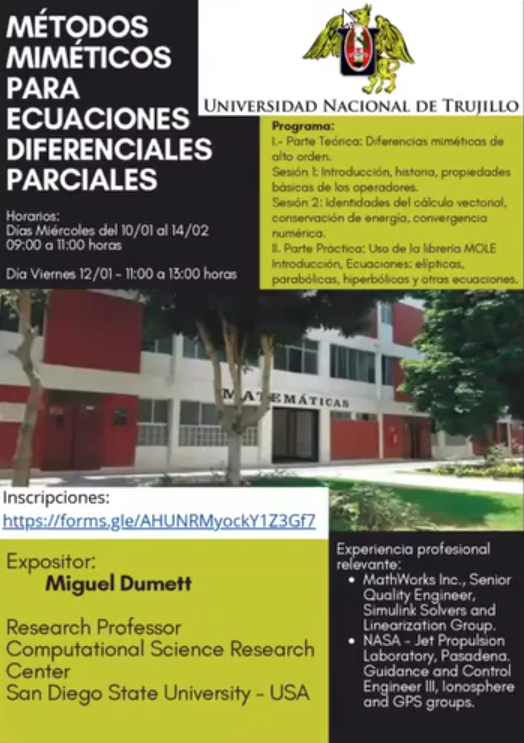
\includegraphics[width=.3\paperwidth]{mole2024}\quad
	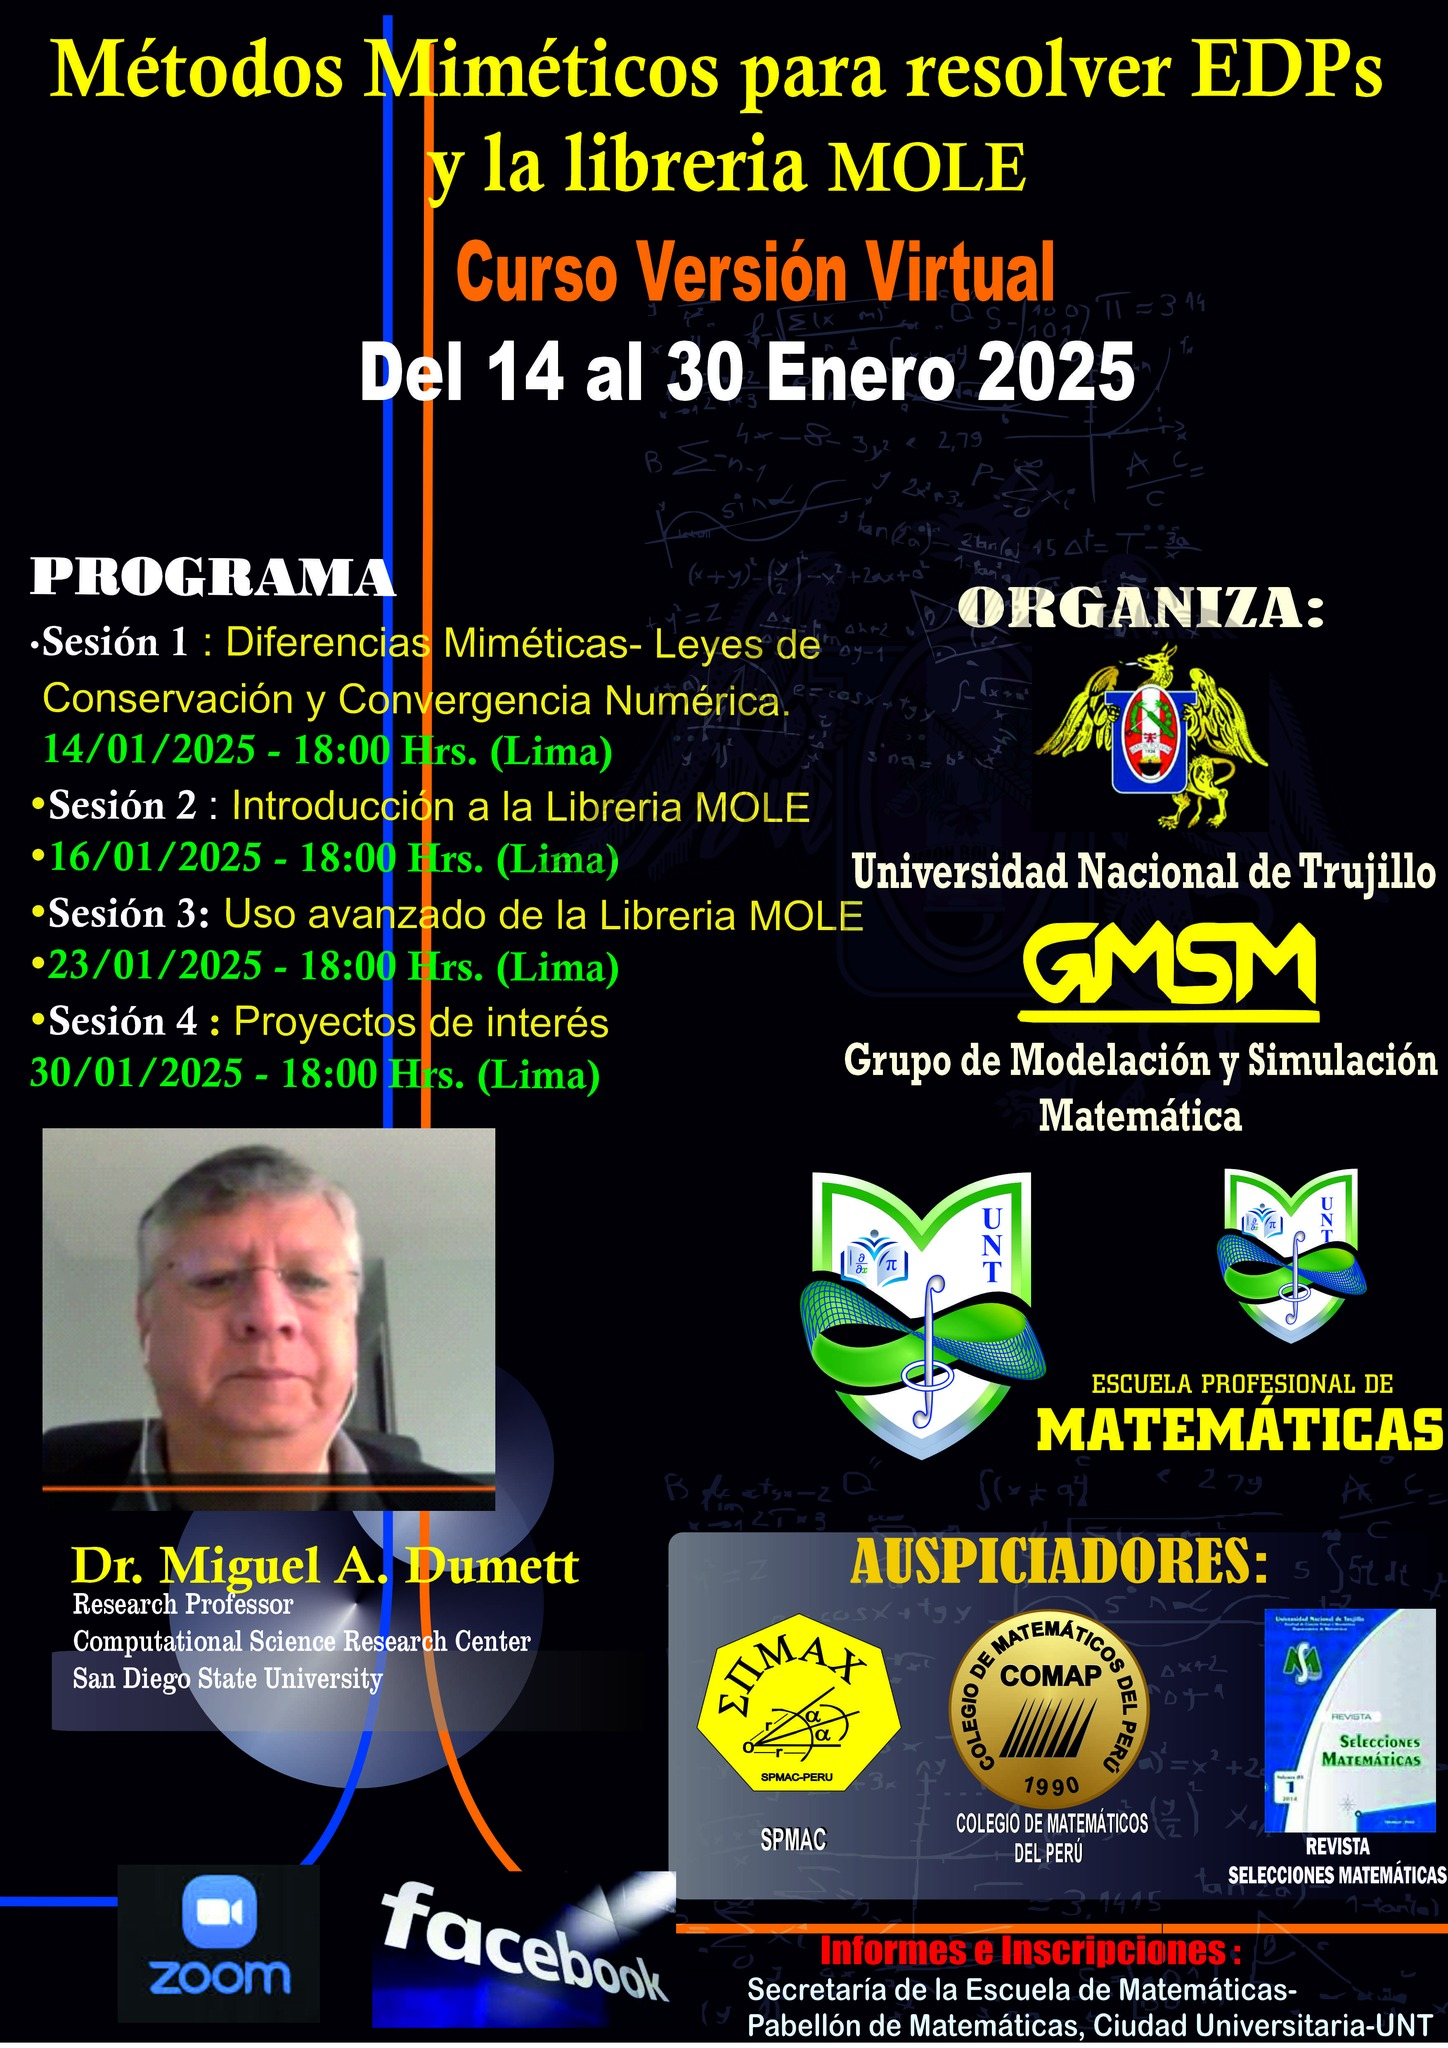
\includegraphics[width=.3\paperwidth]{mole2025}
	\caption*{\bfseries Mimetic Methods courses in January and February 2024 and 2025.}
\end{figure}

